% Tiefpass Amplitudengang (MINIMAL), lineare Achsen, tau = 10 ms
\begin{tikzpicture}[x=1mm,y=1mm] % gilt für tikz-coordinaten außerhalb der axis-environment
    \draw[draw=none] (-14,-12) rectangle (54,22); % Bildrahmen, Koordinatenbezug auf (0,0) des \begin{axis}...\end{axis} pgfplots, für
    \begin{axis}[
        xmode=linear,
        ymode=linear,
        ylabel shift = -5pt,
        ylabel={$A(\omega)$},
        xlabel={$\omega\ [\mathrm{Hz}]$},
        xmin=0, xmax=1e3,
        domain=1e0:1e3, 
        ymin=-0, ymax=1,
        samples=61,
        width=6.5cm,
        height=3.5cm,
        xtick={0,250,500,750,1000},
        xticklabels={0,250,500,750,1000},
        %xtick distance=250,
        ytick distance=0.5,
        yticklabels={,$0$,$\sfrac{1}{2}$,$1$},% first tick label not displayed?
        minor tick num=1,
        grid=both,
        extra x ticks={100},
        extra x tick labels={$\omega_{\mathrm{g}}$},
        extra tick style={grid=none},
        extra y ticks={0.7071},
        %extra y tick labels={$\sqrt[-2]{2}$},
        extra y tick labels={$\sfrac{1}{\sqrt{2}}$},
        extra tick style={grid=none},
        %ytick={0,500,0.7071,1},
        %yticklabels={\ \ \ \0,,$\sqrt{0.5}$,1},
        %xtick distance=250,
        %ytick distance=0.25,
    ]     
        %\addplot[mark=none] coordinates{(0,1)} node[anchor=west,xshift=0pt] {$A(\omega)$};                   % yaxis label in graph
        %\addplot[mark=none] coordinates{(500,0)} node[anchor=center,black,yshift=1pt] {$\omega\ [\mathrm{Hz}]$};      % xaxis label in graph

        \addplot[mark=none,very thick,]   {1/(1+(x*0.01)^2)^0.5}; % 1/(1+(omega*100*100*10^-6)^0.5)^2 % 100 Ohm, 100 uF

    \end{axis}%
\end{tikzpicture}%